% !TEX root = ../termpaper.tex
% first example sections
% @author Thomas Lehmann
%

\section{Grundlagen}
Im folgenden Kapitel wird auf die Grundlagen eingegangen, die in Zusammenhang mit diesem Projekt stehen. Dabei handelt es sich um den bireziproken Teilbandfilter und der Oktav-Filterbank.

\subsection{Bireziproker Teilbandfilter}
Die Grundstruktur des bireziproken Filters sind Wellendigitalfilter. Wellendigitalfilter sind dabei Filter der digitalen Signalverarbeitung, die auch unter nicht linearen Bedingungen eine gute Stabilitätseigenschaft aufweisen \cite[vgl.][S. 68]{gaszi1983}.\par
Bei den bireziproken Filtern, auch selbstreziproke Filter genannt, handelt es sich um eine Unterklasse der Wellendigitalfilter. Bei dem Filterdesign dieser Filter kann entweder die Durchlassdämpfung oder die Sperrdämpfung frei gewählt werden, da der Frequenzbereich bis $\frac{F_s}{4}$ nicht unabhängig von dem Bereich von $\frac{F_s}{4}$ bis $\frac{F_s}{2}$ ist \cite[vgl.][S. 72]{gaszi1983}.\par
Die Anzahl der Adapter innerhalb des Filters ist dabei geringer als bei üblichen Wellendigitalfiltern. Bireziproke Filter umfassen $\frac{N - 1}{2}$ Adapter \cite[vgl.][S. 73]{gaszi1983}.\par
Für dieses Projekt wird der bireziproke Filter aus \cite{gaszi1983} verwendet. Hierbei handelt es sich um einen Filter 19. Grades mit Cauer-Parametern. Das Filterdesign ist in \cite[][S. 74]{gaszi1983} zu finden.\par
Die Struktur des Filters setzt sich wie in Abbildung \ref{fig:bireziprok_Struktur} zusammen.
\begin{figure}[h!]
	\centering	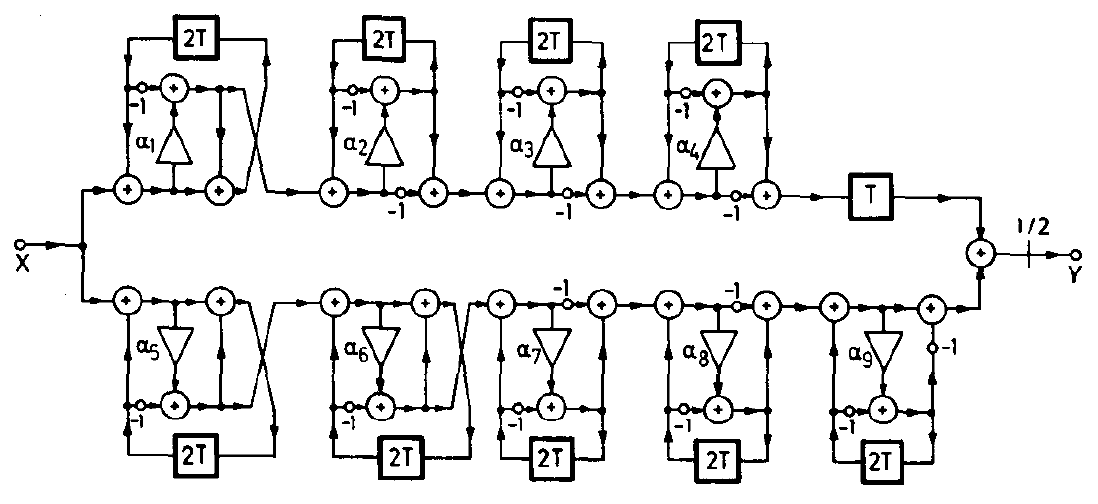
\includegraphics[width=15cm]{img/BireziprokerFilter.png}
	\caption{Struktur des bireziproken Wellendigitalfilters}
	\label{fig:bireziprok_Struktur}
\end{figure}

\subsection{Oktav-Filterbank}